

\section{Traffic Distributions via Weingarten Calculus}
\label{app:weingarten}

We now present different tools and calculations for the traffic distributions of orthogonally invariant matrices based on the \emph{Weingarten formula} for the moments of entries of Haar-random orthogonal matrices.
These essentially follow the ideas of similar calculations by \cite{cebron2024traffic}, but use the version of the Weingarten formula for the orthogonal group, which we review below.

\subsection{Weingarten formula for orthogonal matrices}

For $\bm i = (i_1, \dots, i_k)$ and a perfect matching $\alpha \in \PM([k])$, define
\[ \delta_{\alpha}(\bm i) = \begin{cases} 1 & \text{if } i_u = i_v \text{ for all } \{u, v\} \in \alpha, \\ 0 & \text{otherwise.} \end{cases} \]
The Weingarten calculus expresses the moments of the Haar measure on $O(n)$ in terms of a certain ``Weingarten function'' $W_n(\al, \beta)$ on pairs of matchings.

\begin{lemma}[Weingarten formula]
    Let $\bQ \sim O(n)$ be a Haar-random orthogonal matrix. There exists a function $W_n: \PM([k])^2 \to \R$ such that
    \[
        \E_{\bQ \sim O(n)} \left[\bQ[i_1,j_1]\cdots \bQ[i_k,j_k]\right] = \sum_{\alpha, \beta \in \PM([k])} W_n(\alpha, \beta) \delta_{\alpha}(\bm i) \delta_{\beta}(\bm j).
    \]
\end{lemma}
\noindent
See \cite{CS-2006-HaarMeasureMoments,Banica-2010-OrthogonalWeingartenFormula} for an explicit definition of $W_n(\al, \beta)$.
We will only be interested in asymptotics for $k$ constant and $n \to \infty$, for which the approximations below will suffice.

When $k$ is odd, $\PM([k]) = \varnothing$, so the right-hand side above is zero, and indeed the left-hand side is easily seen to be zero without invoking the Weingarten formula, because $\bQ$ has the same law as $-\bQ$.
So, the only interesting case is $k$ even.
In that case, we give $\PM([k])$ the structure of a metric space, where $\Delta(\alpha, \beta)$ is defined as the minimum number of \emph{swap operations} needed to reach $\beta$ from $\alpha$ (a swap replaces pairs $\{a, b\}$, $\{c, d\}$ with pairs $\{a, c\}$, $\{b, d\}$).
It is easy to check that $\Delta$ is a metric (indeed, it is the distance on a certain graph structure defined on $\PM([k])$).
Further, write $\cyc(\alpha, \beta)$ for the set of even cycles formed by the disjoint union of $\alpha$ and $\beta$.
Then, it is easy to show the alternative characterization
\[ \Delta(\alpha, \beta) = \frac{k}{2} - |\cyc(\alpha, \beta)|\,. \]
As a sanity check, $|\cyc(\alpha, \beta)| \leq \frac{k}{2}$ with equality achieved if and only if $\alpha = \beta$, which is precisely the case $\Delta(\alpha, \beta) = 0$.

For $\alpha, \beta \in \PM([k])$, let $\cP(\alpha, \beta)$ be the set of geodesic paths from $p$ to $q$ in $\PM([k])$, i.e., of sequences $\alpha = \gamma_0, \gamma_1, \dots, \gamma_t = \beta$ with $\gamma_i \neq \gamma_{i + 1}$ for all $i = 0, \dots, t - 1$ and with $\sum_{i = 0}^{t - 1} \Delta(\gamma_i, \gamma_{i + 1}) = \Delta(\alpha, \beta)$.
For such a path $P = (\gamma_0, \dots, \gamma_t)$, write $|P| \colonequals t$.
Then, we define
\begin{align*}
\mu(\al, \beta) 
&= \sum_{P \in \cP(\alpha, \beta)} (-1)^{|P|}
\intertext{This may be viewed as a M{\"o}bius function of the partially ordered set whose chains are geodesics from a given ``base'' matching $p$ to each other matching. An explicit formula from \cite{CS-2006-HaarMeasureMoments} is}
\mu(\al, \beta) &= \prod_{C \in \cyc(\alpha, \beta)} (-1)^{\frac{|C|}{2} - 1}\Cat\left(\frac{|C|}{2} - 1\right) \numberthis \label{eq:cycle-mobius}
\end{align*}
where $\Cat(\cdot)$ are the Catalan numbers.
The key asymptotic for the Weingarten function for our purposes is then the following:

\begin{proposition}[\cite{CS-2006-HaarMeasureMoments}]
\label{lem:weirgarten-asymptotic}
    For a fixed $k$ and $\alpha, \beta \in \PM([k])$, as $n \to \infty$ we have
    \[ W_n(\alpha, \beta) = n^{-k + \cyc(\alpha, \beta)} \left(\mu(\alpha, \beta) + O(n^{-1})\right)\,. \]
\end{proposition}
\noindent
Note that the maximum possible scaling of this quantity is $n^{-k/2}$, which corresponds to the fact that with high probability the entries of $\bQ$ are all roughly of order $n^{-1/2}$.

\subsection{M{\"o}bius inversion on non-crossing partitions}

Recall that $\NC(k)$ is the partially ordered set of non-crossing partitions, i.e., those whose parts do not cross when drawn as a partition of vertices of the $k$-cycle.
We review some standard properties of this partially ordered set; see, e.g., \cite{NS-2006-LecturesCombinatoricsFreeProbability} for a standard reference.

Each non-crossing partition $\pi \in \NC(k)$ has a natural dual partition, called the \emph{Kreweras complement} and denoted $K(\pi)$.
On the cycle graph $C_k$, this may be viewed as the maximal non-crossing partition of the midpoints of the \emph{edges} of $C_k$ that does not cross the boundaries of $\pi$.
Alternatively, one may view both partitions as placed on a single cycle graph of twice the size, $C_{2k}$, on alternating sets of vertices.
We show this viewpoint with an example in~\cref{fig:kreweras}.
The map $K: \NC(k) \to \NC(k)$ is easily checked to be an involution.

\begin{figure}[!htbp]
\begin{center}
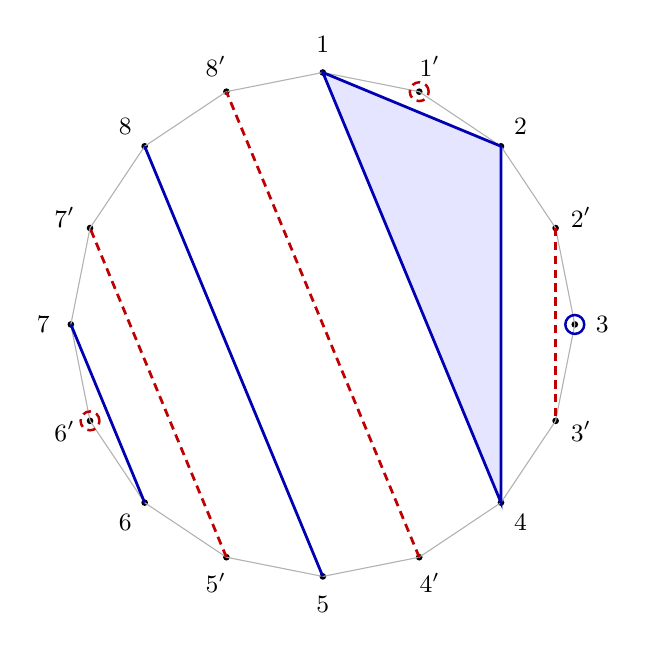
\begin{tikzpicture}[scale=1, every node/.style={font=\small}]
  \def\R{3.2}
  \def\Rlab{3.55}

  \foreach \name/\ang/\lab in {
    u1/90/{$1$},   p1/67.5/{$1'$},
    u2/45/{$2$},   p2/22.5/{$2'$},
    u3/0/{$3$},    p3/-22.5/{$3'$},
    u4/-45/{$4$},  p4/-67.5/{$4'$},
    u5/-90/{$5$},  p5/-112.5/{$5'$},
    u6/-135/{$6$}, p6/-157.5/{$6'$},
    u7/180/{$7$},  p7/157.5/{$7'$},
    u8/135/{$8$},  p8/112.5/{$8'$}
  }{
    \coordinate (\name) at (\ang:\R);
    \fill (\name) circle (1.2pt);
    \node at (\ang:\Rlab) {\lab};
  }

  \draw[gray!60]
    (u1)--(p1)--(u2)--(p2)--(u3)--(p3)--(u4)--(p4)--
    (u5)--(p5)--(u6)--(p6)--(u7)--(p7)--(u8)--(p8)--cycle;

  \filldraw[fill=blue!10, draw=blue!70!black, line width=1pt]
    (u1)--(u2)--(u4)--cycle;
  \draw[blue!70!black, line width=1pt] (u5)--(u8);
  \draw[blue!70!black, line width=1pt] (u6)--(u7);
  \draw[blue!70!black, line width=0.9pt] (u3) circle[radius=0.12];

  \draw[red!75!black, densely dashed, line width=1pt] (p2)--(p3);
  \draw[red!75!black, densely dashed, line width=1pt] (p4)--(p8);
  \draw[red!75!black, densely dashed, line width=1pt] (p5)--(p7);
  \draw[red!75!black, densely dashed, line width=0.9pt] (p1) circle[radius=0.12];
  \draw[red!75!black, densely dashed, line width=0.9pt] (p6) circle[radius=0.12];
\end{tikzpicture}
\end{center}
\caption{An illustration of the Kreweras complement operation on non-crossing partitions. The parts of a partition $\pi \in \NC(8)$ are drawn in blue, and the parts of the Kreweras complement $K(\pi) \in \NC(8)$ in red.}
\label{fig:kreweras}
\end{figure}


We give $\NC(k)$ the usual partial ordering of refinement of partitions, written $\pi \psdleq \rho$, using that a refinement of a non-crossing partition remains non-crossing.
This partial ordering has a minimal element $\underline{0} \in \NC(k)$, the partition where every block is a singleton, and a maximal element $\underline{1} \in \NC(k)$, the partition with just one block.
The Kreweras complement is an \emph{anti-isomorphism} of this ordering: it is a bijection that reverses the ordering, i.e.\ $K(\pi) \preceq K(\rho)$ if and only if $\pi \succeq \rho$.
In particular, $K(\underline{0}) = \underline{1}$ and $K(\underline{1}) = \underline{0}$.

The \Mobius\ function for the $\NC(k)$ poset gives values $\mu(\pi, \rho)$ for each pair $\pi \preceq \rho$.
The Kreweras complement interacts with the \Mobius\ function in the following way that will be crucial for our purposes:
\begin{equation}\label{eq:kreweras-mobius}
\mu(\underline{0}, \pi) = \mu(K(\pi), \underline{1})\,. 
\end{equation}
Further, evaluations of the \Mobius\ function as on the left-hand side may be expanded as products over the blocks of $\pi$, and the factors turn out to be the same as the combinatorial quantities appearing in~\cref{eq:cycle-mobius}; there is a combinatorial explanation for this coincidence but we will just need to use that this indeed occurs:
\[ \mu(\underline{0}, \pi) = \prod_{A \in \pi} (-1)^{|A| - 1} \Cat(|A| - 1)\,. \]

Note that, applying \Mobius inversion to \cref{eq:free-cumulant}, we obtain an explicit formula for the free cumulants in terms of the moments, as mentioned earlier in the main text: if $m_k$ are the moments of a probability measure, then the free cumulants $\kappa_k$ are
\begin{equation} \label{eq:free-cumulant-explicit}
\kappa_k = \sum_{\pi \in \NC(k)} \mu(\pi, \underline{1}_k) \prod_{A \in \pi} m_{|A|}\,. 
\end{equation}




\subsection{Tracial moments concentration}

The result of~\cite{cebron2024traffic} also assumes the following formula for the joint moments of the various trace powers of a matrix, that we also use in our proof.
We show that it follows from our assumptions.

\begin{lemma}[Tracial moments concentration]\label{lem:factorization}
    Let $\bA = \bA^{(n)} \in \R^{n \times n}_\sym$ be  random  matrices that converge in tracial moments in $L^2$ to some $\mu$. Then for any cycle diagrams
    $\rho_1, \ldots, \rho_k$,
    \[
        \lim_{n\to\infty} \E\left[\prod_{j=1}^k \frac 1n w_{\rho_j}(\bmA)\right] = \prod_{j=1}^k \lim_{n\to\infty}  \E \frac 1n w_{\rho_j}(\bmA)\,.
    \]
\end{lemma}

\begin{proof}
    Let us write $T_q = T_q^{(n)} \defeq \frac 1n \Tr \bm A^q$. For
    any finite multiset of integers $\mathcal Q$, we can expand
    \[
        \E \left[\prod_{q\in \calQ} T_{q}\right] - \prod_{q\in \calQ} \E T_{q} = \sum_{\varnothing \neq \calQ'\subseteq \calQ} \E\left[\prod_{q\in \calQ'} (T_{q} - \E T_{q})\right] \prod_{q\in \calQ\setminus \calQ'} \E T_{q}\,.
    \]
    Our goal is now to show that each term in the
    sum over $\mathcal Q'$ converges to $0$ as $n\to\infty$. Fix $\mathcal Q'\subseteq \mathcal Q$ such that $\mathcal Q'\neq\varnothing$, and select an arbitrary element $q_0\in \mathcal Q'$. By Cauchy-Schwarz, we have
    \begin{equation}
        \left(\E\left[\prod_{q\in \calQ'} (T_{q} - \E T_{q})\right]\right)^2 \le \E (T_{q_0} - \E T_{q_0})^2 \cdot \E \left[\prod_{q\in \calQ'\setminus \{q_0\}} (T_q - \E T_q)^2\right]\,.\label{eq:tracialBound}
    \end{equation}
    We know that $\E (T_{q_0} - \E T_{q_0})^2$
    converges to $0$ as $n\to\infty$
    by the $L^2$ tracial moments convergence assumption.  For the remaining product of expectations from~\cref{eq:tracialBound}, we apply
    the bound $T_q^2\le T_{2p}^{q/p}$ for all $q\le p$ to get: for all $\mathcal Q''\subseteq \mathcal Q'$,
    \[
        \prod_{q\in \mathcal Q''} T_q^2\le T_{2\sum_{q\in \mathcal Q''} q}\,.
    \]
    Therefore, all terms in the expansion of~\cref{eq:tracialBound} can be bounded
    by products of terms of the form $\E T_q$ for
    $q\in\N$. These are all bounded as $n\to\infty$, since convergence in $L^2$ 
    also implies convergence in expectation.
    Together, we deduce
    \[
        \lim_{n\to\infty} \E \left[\prod_{q\in \calQ} T_{q}\right] = \prod_{q\in \calQ} \lim_{n\to\infty}\E T_{q}\,,
    \]
    which is equivalent to the desired statement.
\end{proof}

\begin{remark}
    \label{rem:cdm-factorization}
    This property is a statement about concentration of the tracial moments.
    For an example where it does not hold, one can take $\bA^{(n)} = a\bm I_n$ for $a \sim \Unif(\{\pm 1\})$, in which case $\lim_{n \to \infty}\EE \frac{1}{n}\Tr(\bA) = \lim_{n \to \infty} \EE \frac{1}{n}\Tr(\bA^3) = 0$, while $\lim_{n \to \infty} \EE [\frac{1}{n}\Tr(\bA) \cdot \frac{1}{n}\Tr(\bA^3)] = 1$.
\end{remark}
\noindent
We will further show below that analogous formulas hold for joint moments of elements of the $w$- and $z$-bases of polynomials, not just the cycle diagrams.

\subsection{Traffic distribution of orthogonally invariant matrices}

We now prove \cref{thm:moments} by computing the traffic distribution of an orthogonally invariant matrix $\bA$, which we recall consists of the limits of expressions of the form $\frac{1}{n}\EE z_{\alpha}(\bA)$ for $\alpha \in \cA_0$.

First, for a graph $\alpha = (V(\alpha), E(\alpha))$, define $\mathrm{HE} = \mathrm{HE}(\alpha)$ to be the set of \emph{half-edges} in $\alpha$, a set of size $|\mathrm{HE}| = 2|E|$ which may be identified with pairs $(v, \{v, w\})$ for each choice of $v \in V$ and $\{v, w\} \in E(\alpha)$.
Then, to $\alpha$ itself is associated a distinguished perfect matching $\widetilde{\alpha} \in \PM(\mathrm{HE})$, which matches each pair $(v, \{v, w\})$ and $(w, \{v, w\})$ of half-edges that correspond to the same edge of $\alpha$ (this is the perfect matching that would realize $\alpha$ under the configuration model).

We say that a matching $\beta \in \calM(\mathrm{HE})$ is \emph{$\alpha$-local} if all of its matches are between half-edges of the form $(v, e_1)$, $(v, e_2)$, i.e., between pairs of half-edges associated to the same \emph{vertex} (rather than the same \emph{edge}) for $\widetilde{\alpha}$.
Let $\Loc(\alpha) \subseteq \PM(\mathrm{HE}(\alpha))$ be the set of all $\alpha$-local matchings.
Note that $\Loc(\alpha) \neq \varnothing$ if and only if $\alpha$ is Eulerian, i.e., if every vertex has even degree.

At the heart of the matter is the distance between $\widetilde{\alpha}$ and the set $\Loc(\alpha)$, which is minimized precisely by the cactus graphs $\alpha\in\calC$:
\begin{proposition}
    \label{prop:cactus-loc-dist}
    For any graph $\alpha$, not necessarily connected, all of whose connected components are Eulerian, we have
    \[ \Delta(\widetilde{\alpha}, \Loc(\alpha)) = \min_{\beta \in \Loc(\alpha)} \Delta(\widetilde{\alpha}, \beta) \geq |V(\alpha)| - |\conn(\alpha)|\,, \]
    with equality if and only if every connected component of $\alpha$ is a cactus.
    Further, in that case, there is a unique $\beta \in \Loc(\alpha)$ achieving equality, which is the (unique) such $\beta$ that matches pairs of half-edges belonging to the same cycle in $\alpha$.
\end{proposition}
\begin{proof}
    It suffices to consider $\alpha$ connected; the general case follows by considering each connected component separately.

    We may rewrite
    \begin{align*}
    \Delta(\widetilde{\alpha}, \Loc(\alpha)) 
    &= \min_{\beta \in \Loc(\alpha)} \Delta(\widetilde{\alpha}, \beta) = |E| - \max_{\beta \in \Loc(\alpha)} |\cyc(\widetilde{\alpha}, \beta)|
    \end{align*}
    and therefore it suffices to show that, for all $\alpha$-local matchings of half-edges $\beta$, we have
    \[ |\cyc(\widetilde{\alpha}, \beta)| \stackrel{\text{(?)}}{\leq} |E| - |V| + 1\,. \]
    The set of cycles in the disjoint union of $\widetilde{\alpha}$ and an $\alpha$-local $\beta$ is equivalently the number of cycles in a cycle cover of $\alpha$ (i.e., a partition of its edges into cycles).

    The bound is tight for cycles.
    Suppose $C_1, \dots, C_k$ is a cycle cover of some connected multigraph $\alpha$.
    Since $\alpha$ is connected, it is possible to order the $C_i$ such that $C_{i + 1}$ has a vertex in common with the union of $C_1, \dots, C_i$ for each $i = 1, \dots, k - 1$.
    Adding each successive $C_i$ then increases $|E| - |V| + 1$ by at least 1, so the bound follows.
    If the bound is tight, then in the above ordering $C_{i + 1}$ must have exactly one vertex in common with the union of $C_1, \dots, C_i$, and thus is a cactus.
    In that case, there is only one cycle cover, and thus the minimizer $\beta$ is unique and must be as specified in the statement.
\end{proof}

\begin{figure}
\begin{center}
\begin{tikzpicture}[
  x=1cm,y=1cm,
  halfedge/.style={circle,fill=black,inner sep=1.5pt},
  alphamatch/.style={draw=blue!70!black,line width=1.1pt},
  betamatch/.style={draw=red!75!black,line width=1.1pt},
  blob/.style={fill=gray!18,draw=gray!45,rounded corners=5pt,inner sep=5pt}
]

\coordinate (c)  at ( 0.0,  3.0);
\coordinate (a1) at (-4.1,  1.7);
\coordinate (b1) at (-2.0,  0.7);
\coordinate (a2) at (-0.9, -0.9);
\coordinate (b2) at ( 1.0, -0.9);
\coordinate (a3) at ( 3.0,  2.7);
\coordinate (b3) at ( 1.8,  0.7);
\coordinate (x)  at (-6.3,  0.9);
\coordinate (y)  at (-6.1, -1.5);
\coordinate (z)  at (-3.8, -1.7);

\coordinate (hcAone)  at ($(c)!7mm!(a1)$);
\coordinate (hcBone)  at ($(c)!7mm!(b1)$);
\coordinate (haonec)  at ($(a1)!7mm!(c)$);
\coordinate (haoneb)  at ($(a1)!7mm!(b1)$);
\coordinate (hb1a1)   at ($(b1)!6mm!(a1)$);
\coordinate (hb1c)    at ($(b1)!6mm!(c)$);

\coordinate (hcAtwo)  at ($(c)!7mm!(a2)$);
\coordinate (hcBtwo)  at ($(c)!7mm!(b2)$);
\coordinate (hatwoc)  at ($(a2)!6mm!(c)$);
\coordinate (hatwob)  at ($(a2)!6mm!(b2)$);
\coordinate (hb2a2)   at ($(b2)!6mm!(a2)$);
\coordinate (hb2c)    at ($(b2)!6mm!(c)$);

\coordinate (hcAthree) at ($(c)!7mm!(a3)$);
\coordinate (hcBthree) at ($(c)!7mm!(b3)$);
\coordinate (hathreec) at ($(a3)!6mm!(c)$);
\coordinate (hathreeb) at ($(a3)!6mm!(b3)$);
\coordinate (hb3a3)    at ($(b3)!6mm!(a3)$);
\coordinate (hb3c)     at ($(b3)!6mm!(c)$);

\coordinate (haonex)  at ($(a1)!6mm!(x)$);
\coordinate (haonez)  at ($(a1)!6mm!(z)$);
\coordinate (hxa1)    at ($(x)!6mm!(a1)$);
\coordinate (hxy)     at ($(x)!6mm!(y)$);
\coordinate (hyx)     at ($(y)!6mm!(x)$);
\coordinate (hyz)     at ($(y)!6mm!(z)$);
\coordinate (hzy)     at ($(z)!6mm!(y)$);
\coordinate (hza1)    at ($(z)!6mm!(a1)$);

\begin{scope}[on background layer]
  \node[blob,fit=(hcAone)(hcBone)(hcAtwo)(hcBtwo)(hcAthree)(hcBthree)] {};
  \node[blob,fit=(haonec)(haoneb)(haonex)(haonez)] {};
  \node[blob,fit=(hb1a1)(hb1c)] {};
  \node[blob,fit=(hatwoc)(hatwob)] {};
  \node[blob,fit=(hb2a2)(hb2c)] {};
  \node[blob,fit=(hathreec)(hathreeb)] {};
  \node[blob,fit=(hb3a3)(hb3c)] {};
  \node[blob,fit=(hxa1)(hxy)] {};
  \node[blob,fit=(hyx)(hyz)] {};
  \node[blob,fit=(hzy)(hza1)] {};
\end{scope}


\draw[alphamatch] (hcAone)   -- (haonec);
\draw[alphamatch] (haoneb)   -- (hb1a1);
\draw[alphamatch] (hb1c)     -- (hcBone);

\draw[alphamatch] (hcAtwo)   -- (hatwoc);
\draw[alphamatch] (hatwob)   -- (hb2a2);
\draw[alphamatch] (hb2c)     -- (hcBtwo);

\draw[alphamatch] (hcAthree) -- (hathreec);
\draw[alphamatch] (hathreeb) -- (hb3a3);
\draw[alphamatch] (hb3c)     -- (hcBthree);

\draw[alphamatch] (haonex)   -- (hxa1);
\draw[alphamatch] (hxy)      -- (hyx);
\draw[alphamatch] (hyz)      -- (hzy);
\draw[alphamatch] (hza1)     -- (haonez);

\draw[betamatch] (hcAone)    -- (hcBone);
\draw[betamatch] (hcAtwo)    -- (hcBtwo);
\draw[betamatch] (hcAthree)  -- (hcBthree);

\draw[betamatch] (haonec)    -- (haoneb);
\draw[betamatch] (haonex)    -- (haonez);

\draw[betamatch] (hb1a1)     -- (hb1c);
\draw[betamatch] (hatwoc)    -- (hatwob);
\draw[betamatch] (hb2a2)     -- (hb2c);
\draw[betamatch] (hathreec)  -- (hathreeb);
\draw[betamatch] (hb3a3)     -- (hb3c);
\draw[betamatch] (hxa1)      -- (hxy);
\draw[betamatch] (hyx)       -- (hyz);
\draw[betamatch] (hzy)       -- (hza1);

\foreach \p in {
  hcAone,hcBone,haonec,haoneb,hb1a1,hb1c,
  hcAtwo,hcBtwo,hatwoc,hatwob,hb2a2,hb2c,
  hcAthree,hcBthree,hathreec,hathreeb,hb3a3,hb3c,
  haonex,haonez,hxa1,hxy,hyx,hyz,hzy,hza1}
  \node[halfedge] at (\p) {};
\end{tikzpicture}
\end{center}
\caption{An illustration of the matchings involved in~\cref{prop:cactus-loc-dist} and the arguments afterwards. Gray regions represent vertices of a cactus graph $\alpha$, three triangles joined at a vertex with one 4-cycle attached to one of those triangles at a different vertex. This graph has $|V| = 10$ and $|E| = 13$. Black dots in those regions represent half-edges of $\alpha$. In blue, we draw the matching $\widetilde{\alpha}$ realizing the graph $\alpha$; if the gray regions are each contracted to a point and only blue edges are retained, then the resulting graph is the cactus $\alpha$. In red, we draw the unique $\alpha$-local matching $\beta$ that maximizes $|\cyc(\widetilde{\alpha}, \beta)| = |E| - |V| + 1 = 4$; its being $\alpha$-local corresponds to making matches only within the gray regions.}
\label{fig:matchings}
\end{figure}

We now proceed to \Cref{thm:moments} by calculating the traffic distribution of a sequence of orthogonally invariant random matrices $\bA = \bA^{(n)}$.
We could view this as $\bA = \bQ\bD\bQ^{\top}$ for a Haar-distributed orthogonal $\bQ$ and some random diagonal $\bD$, but actually this will not be necessary.
Instead, let us take a perspective similar to the calculations in, for instance, \cite{KMW-2024-TensorCumulantsInvariantInference}, which we believe is useful in general.
Our idea will be to average the $z_{\alpha}(\bA)$ over a random rotation $\bQ$ drawn independently of $\bA$.
Regardless of the structure of $\bA$, this defines another family of polynomials:
\[ \bar{z}_{\alpha}(\bA) \colonequals \E_{\bQ} z_{\alpha}(\bQ\bA\bQ^{\top})\,. \]
If $\bQ$ is drawn from Haar measure, then the $\bar{z}_{\alpha}$ will be orthogonally invariant polynomials, a greater symmetry than permutation invariance of $z_{\alpha}$.
In particular, since the invariants of matrices under the $O(n)$ action are generated by traces of matrix powers, $\bar{z}_{\alpha}$ will be a polynomial in these.

\begin{proof}[Proof of \Cref{thm:moments}]
    Let $\bQ \in O(n)$ be Haar-distributed and independent of $\bA$, and let $\alpha = (V, E)$ be a graph.
    As above, write $\mathrm{HE} = \mathrm{HE}(\alpha)$ for the set of half-edges.
    We start by directly expanding the averaged polynomial $\bar{z}$ introduced above:
\begin{align*}
    &\bar{z}_{\alpha}(\bA) \\
    &= \E_{\bQ} z_{\alpha}(\bQ\bA\bQ^{\top}) \\
    &= \E_{\bQ} \sum_{i: V \into [n]} \prod_{\{v, w\} \in E} (\bQ\bA\bQ^{\top})[i(v),i(w)] \\
    &= \E_{\bQ} \sum_{i: V \into [n]} \prod_{\{v, w\} \in E} \left(\sum_{j_1, j_2 = 1}^n \bQ[i(v),j_1] \bA[j_1,j_2] \bQ[i(w),j_2]\right) \\
    &= \E_{\bQ} \sum_{\substack{i: V \into [n] \\ j: \mathrm{HE} \to [n]}} \prod_{\{v, w\} \in E} \bQ[i(v), j(v, \{v, w\})] \bQ[i(w), j(w, \{v, w\})] \bA[j(v, \{v, w\}), j(w, \{v, w\})] \\ 
    &= \sum_{\substack{i: V \into [n] \\ j: \mathrm{HE} \to [n]}} \left( \E_{\bQ} \prod_{\{v, w\} \in E} \bQ[i(v), j(v, \{v, w\})] \bQ[i(w), j(w, \{v, w\})] \right) \\ &\hspace{2.35cm} \cdot \prod_{\{v, w\} \in E}\bA[j(v, \{v, w\}), j(w, \{v, w\})] 
    \intertext{Here, we may use the Weingarten calculus, viewing the matchings involved as matchings of half-edges, provided that we view $i: V \to [n]$ as extended to $i^{\prime}: \mathrm{HE} \to [n]$ by $i'(v, e) \colonequals i(v)$, i.e., labelling a half-edge by the vertex involved. This gives:}
    &= \sum_{\substack{i: V \into [n] \\ j: \mathrm{HE} \to [n]}} \sum_{\beta, \gamma \in \PM(\mathrm{HE})} W(\beta, \gamma) \delta_{\beta}(i^{\prime}) \delta_{\gamma}(j) \prod_{\{v, w\} \in E}\bA[j(v, \{v, w\}), j(w, \{v, w\})] \\
    &= \sum_{j: \mathrm{HE} \to [n]} \sum_{\beta, \gamma \in \PM(\mathrm{HE})} \left(\sum_{i: V \into [n]} \delta_{\beta}(i^{\prime})\right) W(\beta, \gamma) \delta_{\gamma}(j) \prod_{\{v, w\} \in E}\bA[j(v, \{v, w\}), j(w, \{v, w\})]
    \intertext{The summation over $i$ is zero unless $\beta \in \Loc(\alpha)$, and in that case each choice of $i$ contributes 1, for a total of $n^{|V|}(1 + O(n^{-1}))$. So, we have}
    &= \left(1 + O\left(\frac{1}{n}\right)\right)n^{|V|} \sum_{\gamma \in \PM(\mathrm{HE})} \left(\sum_{\beta \in \Loc(\alpha)} W(\beta, \gamma)\right) \\
    &\hspace{3.95cm}\sum_{j:\textnormal{ HE} \to [n]} \delta_{\gamma}(j) \prod_{\{v, w\} \in E}\bA[j(v, \{v, w\}), j(w, \{v, w\})]
    \intertext{The remaining summation may be grouped into summations over the cycles in the disjoint union of $\gamma$ and $\widetilde{\alpha}$, which gives}
    &= \left(1 + O\left(\frac{1}{n}\right)\right)n^{|V|} \sum_{\gamma \in \PM(\mathrm{HE})} \left(\sum_{\beta \in \Loc(\alpha)} W(\beta, \gamma)\right) \prod_{C \in \cyc(\widetilde{\alpha}, \gamma)} \Tr(\bA^{\frac{|C|}{2}})
    \intertext{Now, we may use the asymptotic formula in \cref{lem:weirgarten-asymptotic} and normalize the traces to get}
    &= \left(1 + O\left(\frac{1}{n}\right)\right)n^{|V|} \sum_{\gamma \in \PM(\mathrm{HE})} \\
    &\hspace{1cm} \left(\sum_{\beta \in \Loc(\alpha)} \left(1 + O\left(\frac{1}{n}\right)\right)n^{-|\mathrm{HE}| + \cyc(\beta, \gamma)} \mu(\beta, \gamma)\right) \prod_{C \in \cyc(\widetilde{\alpha}, \gamma)} \Tr(\bA^{\frac{|C|}{2}}) \\
    &= \left(1 + O\left(\frac{1}{n}\right)\right)n^{|V|} \sum_{\gamma \in \PM(\mathrm{HE})} \\
    &\hspace{1cm} \left(\sum_{\beta \in \Loc(\alpha)} \left(1 + O\left(\frac{1}{n}\right)\right)n^{-|\mathrm{HE}| + \cyc(\beta, \gamma) + \cyc(\widetilde{\alpha}, \gamma)} \mu(\beta, \gamma)\right) \prod_{C \in \cyc(\widetilde{\alpha}, \gamma)} \frac{1}{n}\Tr(\bA^{\frac{|C|}{2}}) \\
    &= \left(1 + O\left(\frac{1}{n}\right)\right)n^{|V|} \sum_{\gamma \in \PM(\mathrm{HE})} \\
    &\hspace{1cm}\left(\sum_{\beta \in \Loc(\alpha)} \left(1 + O\left(\frac{1}{n}\right)\right)n^{-\Delta(\beta, \gamma) - \Delta(\widetilde{\alpha}, \gamma)} \mu(\beta, \gamma)\right) \prod_{C \in \cyc(\widetilde{\alpha}, \gamma)} \frac{1}{n}\Tr(\bA^{\frac{|C|}{2}})\,.
\end{align*}
Let us pause to notice that we have achieved our initial goal, expressing the orthogonally invariant polynomial $\bar{z}_{\alpha}(\bA)$ as a polynomial in traces of powers of $\bA$.
We now use that, if $\bA$ was orthogonally invariant to begin with, then
\[ \E_{\bA} z_{\alpha}(\bA) = \E_{\bA} \bar{z}_{\alpha}(\bA) \]
and continue to determine the right-hand side as $n \to \infty$.

By the triangle inequality, we have
\[ \Delta(\beta, \gamma) + \Delta(\widetilde{\alpha}, \gamma) \geq \Delta(\beta, \widetilde{\alpha}) \geq \Delta(\widetilde{\alpha}, \Loc(\alpha)) \geq |V| - 1\,. \]
Therefore, under our assumptions, all terms are negligible as $n \to \infty$ except for those where equality is achieved throughout above.

By~\Cref{prop:cactus-loc-dist}, we then find that if $\alpha$ is not a cactus then
\[ \lim_{n \to \infty} \frac{1}{n}\E_{\bA} z_{\alpha}(\bA) = 0\,. \]
So, suppose that $\alpha$ is a cactus.
Then, using the factorization property (\cref{lem:factorization}), we have in the limit that
\begin{align*}
    \lim_{n \to \infty} \frac{1}{n}\EE_{\bA} z_{\alpha}(\bA) 
    &= \sum_{\substack{\beta \in \Loc(\alpha) \\ \Delta(\beta, \widetilde{\alpha}) = |V| - 1}} \,\,\, \sum_{\substack{\gamma \in \PM(\mathrm{HE}) \\ \Delta(\beta, \gamma) + \Delta(\gamma, \widetilde{\alpha}) = \Delta(\beta, \widetilde{\alpha})}} \mu(\beta, \gamma) \prod_{C \in \cyc(\widetilde{\alpha}, \gamma)} m_{|C| / 2}
    \intertext{where $m_k$ are the spectral moments. Letting $\eta$ be the $\alpha$-local matching of half-edges belonging to the same cycle around each vertex, by the uniqueness clause of~\Cref{prop:cactus-loc-dist} we further have that only the term $\beta = \eta$ contributes, giving}
    &= \sum_{\substack{\gamma \in \PM(\mathrm{HE}) \\ \Delta(\eta, \gamma) + \Delta(\eta, \widetilde{\alpha}) = \Delta(\eta, \widetilde{\alpha})}} \mu(\eta, \gamma) \prod_{C \in \cyc(\widetilde{\alpha}, \gamma)} m_{|C| / 2}
    \intertext{Suppose there are $k$ cycles in $\alpha$. Then, $|\cyc(\eta, \widetilde{\alpha})| = k$, and, rewriting the condition on $\gamma$ in terms of cycle counts and using the explicit formula for the \Mobius\ function from~\cref{eq:cycle-mobius}, we have}
    &= \sum_{\substack{\gamma \in \PM(\mathrm{HE}) \\ |\cyc(\eta, \gamma)| + |\cyc(\gamma, \widetilde{\alpha})| = |E| + k}} \prod_{C \in \cyc(\eta, \gamma)} (-1)^{\frac{|C|}{2} - 1} \Cat\left(\frac{|C|}{2} - 1\right) \prod_{C \in \cyc(\widetilde{\alpha}, \gamma)} m_{|C| / 2}
    \intertext{Now, we use that all $\gamma$ appearing in the sum must only match half-edges belonging to the same cycle. Since $\eta$ and $\widetilde{\alpha}$ both have this property also, the various sets of cycles above all form partitions of the cycles in $\alpha$. Thus, the entire sum factorizes over the cycles of $\alpha$. Further, those $\gamma$ that are in the sum have both the partitions of $\cyc(\eta, \gamma)$ and $\cyc(\gamma, \widetilde{\alpha})$ corresponding to non-crossing partitions of each cycle of $\alpha$, and these two non-crossing partitions are Kreweras complements of one another.
    Putting together all these combinatorial observations, we find:}
    &= \prod_{C \in \cyc(\alpha)}\left(\sum_{\pi \in \mathrm{NC}(|C|)} \prod_{A \in K(\pi)} (-1)^{|A| - 1} \Cat(|A| - 1) \cdot \prod_{B \in \pi} m_{|B|}\right)\,.
    \intertext{Now we use \cref{eq:kreweras-mobius} and \cref{eq:free-cumulant-explicit}
    to complete the proof:}
    &= \prod_{C \in \cyc(\alpha)}\left(\sum_{\pi \in \mathrm{NC}(|C|)} \mu(\underline{0}_{|C|}, K(\pi)) \cdot \prod_{B \in \pi} m_{|B|}\right) \\
    &= \prod_{C \in \cyc(\alpha)}\left(\sum_{\pi \in \mathrm{NC}(|C|)} \mu(\pi, \underline{1}_{|C|}) \cdot \prod_{B \in \pi} m_{|B|}\right) \\
    &= \prod_{C \in \cyc(\alpha)} \kappa_{|C|}\,,
\end{align*}
where we have at last identified the free cumulants, completing the calculation.
\end{proof}

We also note that, by exactly the same argument but using the disconnected case of \Cref{prop:cactus-loc-dist}, we may equally well calculate suitably normalized limits of the values of \emph{disconnected} diagrams in the $z$-basis, which factorize over their connected components:
\begin{proposition} \label{prop:invariant-disconnected}
    Let $\bA = \bA^{(n)} \in \R^{n \times n}_{\sym}$ be a sequence of orthogonally invariant random matrices that converge in tracial moments in $L^2$ to a probability measure $\mu$.
    Let $\calD$ denote their limiting traffic distribution, which exists by \Cref{thm:moments} and is given by the explicit formula stated there.
    Then, for all $k \geq 1$ and $\alpha_1, \dots, \alpha_k \in \cA$,
    \[ \lim_{n \to \infty} \frac{1}{n^k} \E z_{\alpha_1 \sqcup \cdots \sqcup \alpha_k}(\bA) = \prod_{i = 1}^k \calD(\alpha_i)\,. \]
\end{proposition}

\subsection{Concentration of traffic observables}

As a corollary, we may also conclude that the traffic distribution is concentrated in the sense of \Cref{def:traffic-concentration}.
This also extends {\cite[Theorem 4.7]{cebron2024traffic}} to orthogonally invariant distributions.
\begin{lemma}
    \label{lemma:full-factorization}
    Let $\bmA=\bmA^{(n)}$ be orthogonally invariant random matrices that converge in tracial moments in $L^2$ to a probability measure $\mu$.
    Then the traffic distribution concentrates for $\bA$ (in the sense of \cref{def:traffic-concentration}).
\end{lemma}
\begin{proof}
    Let $k\ge 2$ and $\alpha_1,\ldots,\alpha_k\in \calA$. Then, by \Cref{lem:concentration-z}, it suffices to show the concentration property in the $z$-basis, namely that:
    \begin{align*}
        \lim_{n\to\infty} \E\left[\prod_{i=1}^k \frac 1n z_{\alpha_i}(\bmA)\right] 
        \stackrel{\text{(?)}}{=} \lim_{n\to\infty} \prod_{i=1}^k \E \frac 1n z_{\alpha_i}(\bmA)\,.
    \end{align*}

    Note that, upon expanding the summations in the $z$-basis polynomials, we have
    \[ z_{\alpha_1}(\bA) \cdots z_{\alpha_k}(\bA) = z_{\alpha_1 \sqcup \cdots \sqcup \alpha_k}(\bA) + z_{\beta_1}(\bA) + \cdots + z_{\beta_M}(\bA)\,, \]
    where $\alpha_1 \sqcup \cdots \sqcup \alpha_k$ is the disjoint union, while the $\beta_i$ are various graphs formed by identifying subsets of the vertices of this disjoint union according to different non-trivial partitions of the vertices, provided that no two vertices of the same $\alpha_j$ are identified.
    In particular, all $\beta_i$ have at most $k - 1$ connected components.
    Therefore, by \Cref{prop:invariant-disconnected}, we have
    \[ \lim_{n \to \infty} \frac{1}{n^k} z_{\beta_i}(\bA) = 0 \]
    for all $i \in [M]$.
    Thus, 
    \[ \lim_{n \to \infty} \frac{1}{n^k}\E\left[\prod_{i=1}^k z_{\alpha_i}(\bmA)\right] = \lim_{n \to \infty} \frac{1}{n^k}\E[z_{\alpha_1 \sqcup \cdots \sqcup \alpha_k}(\bA)]\,, \]
    and the result then follows by \Cref{prop:invariant-disconnected}.
\end{proof}

\subsection{Traffic distribution of punctured orthogonally invariant matrices}
\label{sec:puncturedWeingarten}

Since the \rrom plays an important role in our main results, let us sketch how similar calculations can give an explicit combinatorial description of its traffic distribution, and indeed that of the puncturing of any orthogonally invariant random matrices.
Recall that in the main text we relied entirely on the implicit description of this traffic distribution via \Cref{lem:eqDiffMobius}.
The closed form we give below is completely explicit, but, being in terms of a rather complicated summation over matchings, seems less useful than the implicit one.

We follow the notation from the proof in the previous section.
Additionally, for a graph $\alpha$ and a matching $\beta$ of the half-edges of $\alpha$, we write $\loc(\beta)$ for the set of edges of $\beta$ that go between half-edges of the same vertex of $\alpha$, and $\nonloc(\beta)$ for the set of edges of $\beta$ that go between half-edges of different vertices of $\alpha$.
Recall also that $\widetilde{\alpha}$ is the matching of half-edges of $\alpha$ corresponding to the edges actually in the graph $\alpha$.
\begin{theorem}
    Let $\bA = \bA^{(n)} \in \R^{n \times n}_\sym$ be a sequence of orthogonally invariant random matrices that converges in tracial moments in $L^2$ to a probability measure $\mu$.
    Write $m_k$ for the $k$th moment of $\mu$ and $\bm\Pi = \bm\Pi^{(n)} = \bm I - \frac{1}{n}\bm 1 \bm 1^{\top}$.
    Then, for all $\al \in \calA$,
    \[ \lim_{n \to \infty} \frac{1}{n}\EE_{\bA} z_{\alpha}(\bm \Pi\bA\bm \Pi) = \sum_{\substack{\beta \in \PM(\mathrm{HE}(\alpha)) \\ \alpha \sqcup \nonloc(\beta) \text{ is a cactus}}} (-1)^{|\nonloc(\beta)|} \sum_{\substack{\gamma \in \PM(\mathrm{HE}(\alpha)) \\ \Delta(\beta, \gamma) + \Delta(\gamma, \widetilde{\alpha}) = \Delta(\beta, \widetilde{\alpha})}} \mu(\beta, \gamma) \prod_{C \in \cyc(\widetilde{\alpha}, \gamma)} m_{|C|}\,. \]
\end{theorem}
\begin{proof}
Following the same calculations as in the proof of \Cref{thm:moments} above but now applied to $\bm\Pi \bQ\bA\bQ^{\top}\bm\Pi$, we instead find:
\begin{align*}
    &\frac{1}{n}\EE_{\bQ, \bA} z_{\alpha}(\bm\Pi\bQ\bA\bQ^{\top}\bm\Pi) \\
    &= \frac{1}{n}\EE_{\bA}\sum_{\beta, \gamma \in \PM(\mathrm{HE})} W_n(\beta, \gamma) \cdot \prod_{C \in \cyc(\widetilde{\alpha}, \gamma)} \Tr(\bA^{|C|}) \cdot z_{G(\beta)}(\bm\Pi)
    \intertext{where $G(\beta)$ denotes the graph formed by ``wiring together'' the matching of half-edges $\beta$ (so that, for example, $G(\widetilde{\alpha}) = \alpha$). Note that here if we replaced $\bm\Pi$ by $\bm I$, we would get $z_{G(\beta)}(\bm I) = \mathbf 1_{\beta \in \Loc(\alpha)} n^{|V|}(1+O(n^{-1}))$, compatible with the previous calculation in the proof of \Cref{thm:moments}, and indeed the above is true for an arbitrary symmetric matrix $\bm\Pi$, not only the particular projection we are concerned with. But, in our particular case, since $\bm\Pi$ is constant on the diagonal and on the off-diagonal, we have}
    &= \frac{1}{n}\sum_{\beta, \gamma \in \PM(\mathrm{HE})} W_n(\beta, \gamma) \cdot \EE_{\bA}\prod_{C \in \cyc(\widetilde{\alpha}, \gamma)} \Tr(\bA^{|C|}) \cdot n^{\underline{|V|}}\left(-\frac{1}{n}\right)^{|\nonloc(\beta)|} \left(1 - \frac{1}{n}\right)^{|\loc(\beta)|}
    \intertext{and now by the same asymptotics as before,}
    &= \sum_{\beta, \gamma \in \PM(\mathrm{HE})} 
    \left(1 + O\left(\frac{1}{n}\right)\right) n^{-\Delta(\widetilde{\alpha}, \gamma) - \Delta(\beta, \gamma) - |\nonloc(\beta)| + |V| - 1} \mu(\beta, \gamma) (-1)^{|\nonloc(\beta)|}
     \prod_{C \in \cyc(\widetilde{\alpha}, \gamma)} m_{|C|}
\end{align*}   

We claim that, for any connected $\alpha$ realized by the matching $\widetilde{\alpha}$ of its half-edges, and any other matching $\beta$ of the half-edges of $\alpha$, we have
\[ \Delta(\widetilde{\alpha}, \beta) + |\nonloc(\beta)| \geq |V| - 1\,. \]
As before, this is equivalent to having
\[ |\cyc(\widetilde{\alpha}, \beta)| \leq |E| + |\nonloc(\beta)| - |V| + 1\,. \]
Consider an ancillary graph $\alpha^{\prime}$ constructed by adding edges to $\alpha$ for each non-local match in $\beta$.
This graph is still connected, by parity considerations it must be Eulerian, and it has a total of $|E| + |\nonloc(\beta)|$ edges.
$|\cyc(\widetilde{\alpha}, \beta)|$ is now the size of a cycle cover of $\alpha^{\prime}$, and the claim then follows by the bounds from the proof of~\Cref{prop:cactus-loc-dist} applied to $\alpha^{\prime}$.

We also again have by the triangle inequality that
\[ \Delta(\widetilde{\alpha}, \gamma) + \Delta(\beta, \gamma) \geq \Delta(\widetilde{\alpha}, \beta)\,. \]
Thus, all terms in the sum above are of at most constant order.
Further, those of constant order are those where the exponent of $n$ is zero, which are those where the above bound is tight.
By the characterization in~\Cref{prop:cactus-loc-dist}, this is precisely when $\alpha^{\prime}$ as formed above is a cactus, and the stated result follows after rearranging.
\end{proof}